
\documentclass{article}
\usepackage[T1]{fontenc}
\usepackage{graphicx}
\usepackage{amsmath, amsthm, amssymb}
\usepackage{hyperref}
\usepackage{polski}
\usepackage{minted}

\title{SPRAWOZDANIE - LISTA 2}
\author{Zuzanna Pawlik, 282230}
\date{28.11.2024}
\begin{document}
	\maketitle
	
	\section*{FRAGMENTY KODÓW}
	\subsection*{QUICKSORT}
	Fragment kodu QUICKSORT wraz z funkcją pomocniczą PARTITION:
	\begin{minted}{c}
		int PARTITION(int A[], int p, int k){
			int x = A[k];
			int i = p - 1;
			for(int j = p; j < k; j++){
				if(A[j] <= x){
					i++;
					swap(A[i],A[j]);
				}
			}
			swap(A[k],A[i+1]);
			return(i+1);
		}
		
		
		void QUICK_SORT(int A[],int p, int k){
			if(p<k){
				int s = PARTITION(A,p,k);
				QUICK_SORT(A,p,s-1);
				QUICK_SORT(A,s+1,k);
			}
		}
	\end{minted}
	Fragment kody zmodyfikowanego QUICKSORTA, który wykorzystuje 2 uporządkowane pivoty do podziału tablicy, tym samym dzieląc ją na trzy części (zamiast dwóch jak we wcześniejszej wersji). Pomocnicza funkcja PARTITION (zmodyfikowana) zwraca tym razem dwa punkty podziału tablicy:
	\begin{minted}{c}
		void PARTITION_ZMOD(int A[], int p, int k, int& s1, int& s2){
			if(A[p]>A[k]){
				swap(A[p],A[k]);
			}
			
			int x1 = A[p];
			int x2 = A[k];
			int i1 = p + 1;
			int i2 = k - 1;
			
			for(int j = p+1; j <= i2; j++){
				if(A[j] < x1){
					swap(A[i1],A[j]);
					i1++;
				}else if(A[j] > x2){
					swap(A[j],A[i2]);
					i2--;
					j--;
				}
			}
			swap(A[p],A[i1-1]);
			swap(A[k],A[i2+1]);
			s1 = i1-1;
			s2 = i2+1;
		}
		
		void QUICK_SORT_ZMOD(int A[], int p, int k){
			if(p<k){
				int s1,s2;
				PARTITION_ZMOD(A,p,k,s1,s2);
				QUICK_SORT_ZMOD(A,p,s1-1);
				QUICK_SORT_ZMOD(A,s1+1,s2-1);
				QUICK_SORT_ZMOD(A,s2+1,k);
			}
		}
	\end{minted}
	
	\subsection*{RADIXSORT}
	Fragment kodu RADIXSORT z wykorzystaniem COUNTINGSORT. Dodatkowy parametr $d$ w tym algorytmie oznacza system liczbowy, np 2 dla binarnego, czy 10 dla dziesiętnego.
	Ponieważ funkcja ta sortuje po kolejnych cyfrach (zaczynając od jedności) w tej wersji sortuje ona wyłącznie liczby dodatnie.
	\begin{minted}{c}
		void COUNTING_SORT(int A[], int B[], int n, int k, int d){
			int C[d] = {0};
			
			for(int j = 0; j < n; j++){
				C[(A[j]/k)%d]++;
			}
			
			for(int i = 1; i < d; i++){
				C[i] += C[i-1];
			}
			
			for(int j = n-1; j >= 0; j--){
				B[C[(A[j]/k) % d] -1] = A[j];
				C[(A[j]/k) % d]--;
			}
			
			for (int i = 0; i < n; i++) {
				A[i] = B[i];
			}
			
		}
		
		void RADIX_SORT(int A[], int n, int d){
			int max = MAX(A,n);
			int B[n];
			for(int k = 1; max/k > 0; k *= d){
				COUNTING_SORT(A,B,n,k,d);
			}
		}
	\end{minted}
	Poniższa modyfikacja algorytmu RADIXSORT pozwala na sortowanie zarówno liczb ujemnych, jak i dodatnich. Wykorzystuje ona nadal COUNTINGSORT jak wyżej, ale w tej wersji najpierw odpowiednio modyfikujemy dane, aby uzyskać dobre wyniki. Funkcja ta wykorzystuje pomocnicze MIN, które zwraca najmniejszy element tablicy. Jeżeli najmniejszy element jest nieujemny to algorytm wykonuje się jak wyżej. W przeciwnym wypadku od każdego elementu tablicy odejmujemy wartość minimalną (odejmujemy bo $min < 0$), dzięki czemu wszystkie wartości są nieujemne. Następnie tablica jest sortowana jak wyżej. Po posortowaniu do każdego elementu tablicy dodajemy $min$, dzięki czemu przywracamy oryginalne wartości. Operacje te jednak wydłużają czas działania algorytmu (wykonują się dodatkowe przypisania).
	\begin{minted}{c}
		void RADIX_SORT_ZMOD(int A[], int n, int d){
			int min = MIN(A,n);
			if(min>=0){
				int max = MAX(A,n);
				int B[n];
				for(int k = 1; max/k > 0; k*=d){
					COUNTING_SORT(A,B,n,k,d);
				}
			}else{
				for(int i = 0; i < n; i++){
					A[i] = A[i] - min;
				}
				int max = MAX(A,n);
				int B[n];
				for(int k = 1; max/k > 0; k*=d){
					COUNTING_SORT(A,B,n,k,d);
				}
				for(int i = 0; i < n; i++){
					A[i] = A[i] + min;
				}
				
			}
			
		}
		
	\end{minted}
	
	\subsection*{INSERTIONSORT NA LISTACH}
	Poniżej zdefiniowany jest algorytm INSERTIONSORT działający na listach wraz z funkcjami pomocniczymi LISTINSERT i LISTDELETE:
	\begin{minted}{c}
		void LIST_INSERT(Node*& head, Node* x){
			x->next = head;
			x->prev = nullptr;
			if(head != nullptr){
				head->prev = x;
			}
			head = x;
		}
		
		void LIST_DELETE(Node*& head, Node* x){
			if(x->prev != nullptr){
				x->prev->next = x->next;
			}else{
				head = x->next;
			}
			if(x->next != nullptr){
				x->next->prev = x->prev;
			}
			delete x;
		}
		void INSERTION_SORT_LISTY(Node*& head){//I_S na listach
			if(!head || !head->next) return;
			Node* a = head->next;
			while(a != nullptr){
				Node* next = a->next;
				int key = a->key;
				LIST_DELETE(head,a);//usuwamy element ze starego miejsca
				
				Node* posortowana = head;//szukamy miejsca w posortowanej czesci
				while(posortowana != nullptr && posortowana->key < key){//gdzie wstawic
					posortowana = posortowana->next;
				}
				
				Node* Nowy = new Node(key);
				
				if(posortowana == nullptr){//wstawianie na koniec
					Node* tail = head;
					while (tail->next != nullptr) {
						tail = tail->next;
					}
					tail->next = Nowy;
					Nowy->prev = tail;
				}else if(posortowana == head){//wstawianie na poczatek
					LIST_INSERT(head, Nowy);
				}else{//w srodku
					Nowy->next = posortowana;
					Nowy->prev = posortowana->prev;
					if(posortowana->prev != nullptr){
						posortowana->prev->next = Nowy;
					}
					posortowana->prev = Nowy;
				}
				a = next;
			}
		}
	\end{minted}
	\section*{BUCKETSORT}
	Fragment algorytmu BUCKETSORT wykorzystujący powyższy INSERTIONSORT działający na listach (ta wersja działa tylko na liczbach z przedziału $(0,1]$):
	\begin{minted}{c}
		void BUCKET_SORT(double A[], int n){
			List* B = new List[n];
			for(int i = 0; i < n; i++){
				B[i].head = nullptr;
			}
			
			for(int i = 0; i < n; i++){
				int indeksB = min(static_cast<int>(n*A[i]),n-1);
				LIST_INSERT(B[indeksB].head, new Node(A[i]));
			}
			for(int j = 0; j < n; j++){
				INSERTION_SORT_LISTY(B[j].head);
			}
			//przypisanie z B[i] do tablicy A
			int k = 0;//indeksy z tablicy A
			for(int i = 0; i < n; i++){
				Node* a = B[i].head;
				while(a != nullptr){
					A[k] = a->key;
					a = a->next;
					k++;
				}
			}
		}
	\end{minted}
	Modyfikacja BUCKETSORT pozwala na sortowanie dowolnych liczb, a nie tylko z przedziału $(0,1]$. Najpierw wszystkie wartości przesuwamy na dodatnie poprzez odjęcie najmniejszego elementy, następnie dzielimy przez (przesunięty) element największy. Dzięki temu wszystkie wartości możemy sortować jak w powyższym algorytmie. Po posortowaniu zmiany są odwracane. Podobnie jak w przypadku modyfikacji RADIXSORT takie operacje mogą wydłużyć czas działania algorytmu.
	\begin{minted}{c}
		void BUCKET_SORT_ZMOD(double A[], int n){
			double max = MAX(A,n);
			double min = MIN(A,n);
			if(max == min){//wszystkie wartosci takie same - unikanie dzielenia przez 0
				return;
			}else if(0<min && max<=1){//czy wszystkie wartości są z (0,1]
				BUCKET_SORT(A,n); 
			}else{
				for(int i = 0; i < n; i++){
					//najpierw chcemy miec same dodatnie 
					//potem dzieląc przez najwiekszą dostaniemy wartości z (0,1]
					A[i] = (A[i]-min)/(max-min);
				}
				
				BUCKET_SORT(A,n);
				
				for(int i = 0; i < n; i++){//odwracamy zmiany
					A[i] = (A[i]*(max-min))+min;
				}
				
			}
		}
	\end{minted}
	\section*{TABELE I WYKRESY}
	\subsection*{PORÓWNANIE RADIXSORT Z MODYFIKACJĄ}
	\begin{center}
		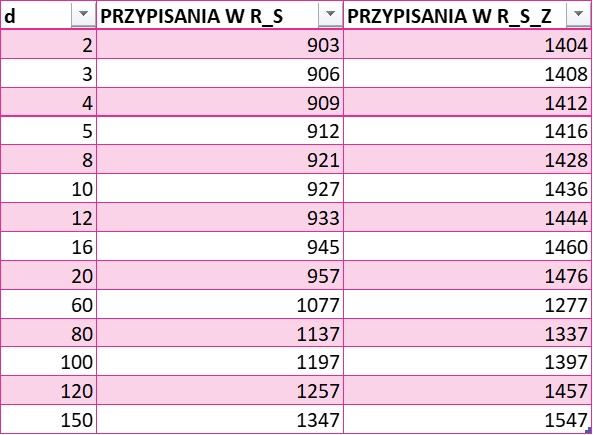
\includegraphics[scale = 0.5]{Obraz1.jpg}
	\end{center}
	\begin{center}
		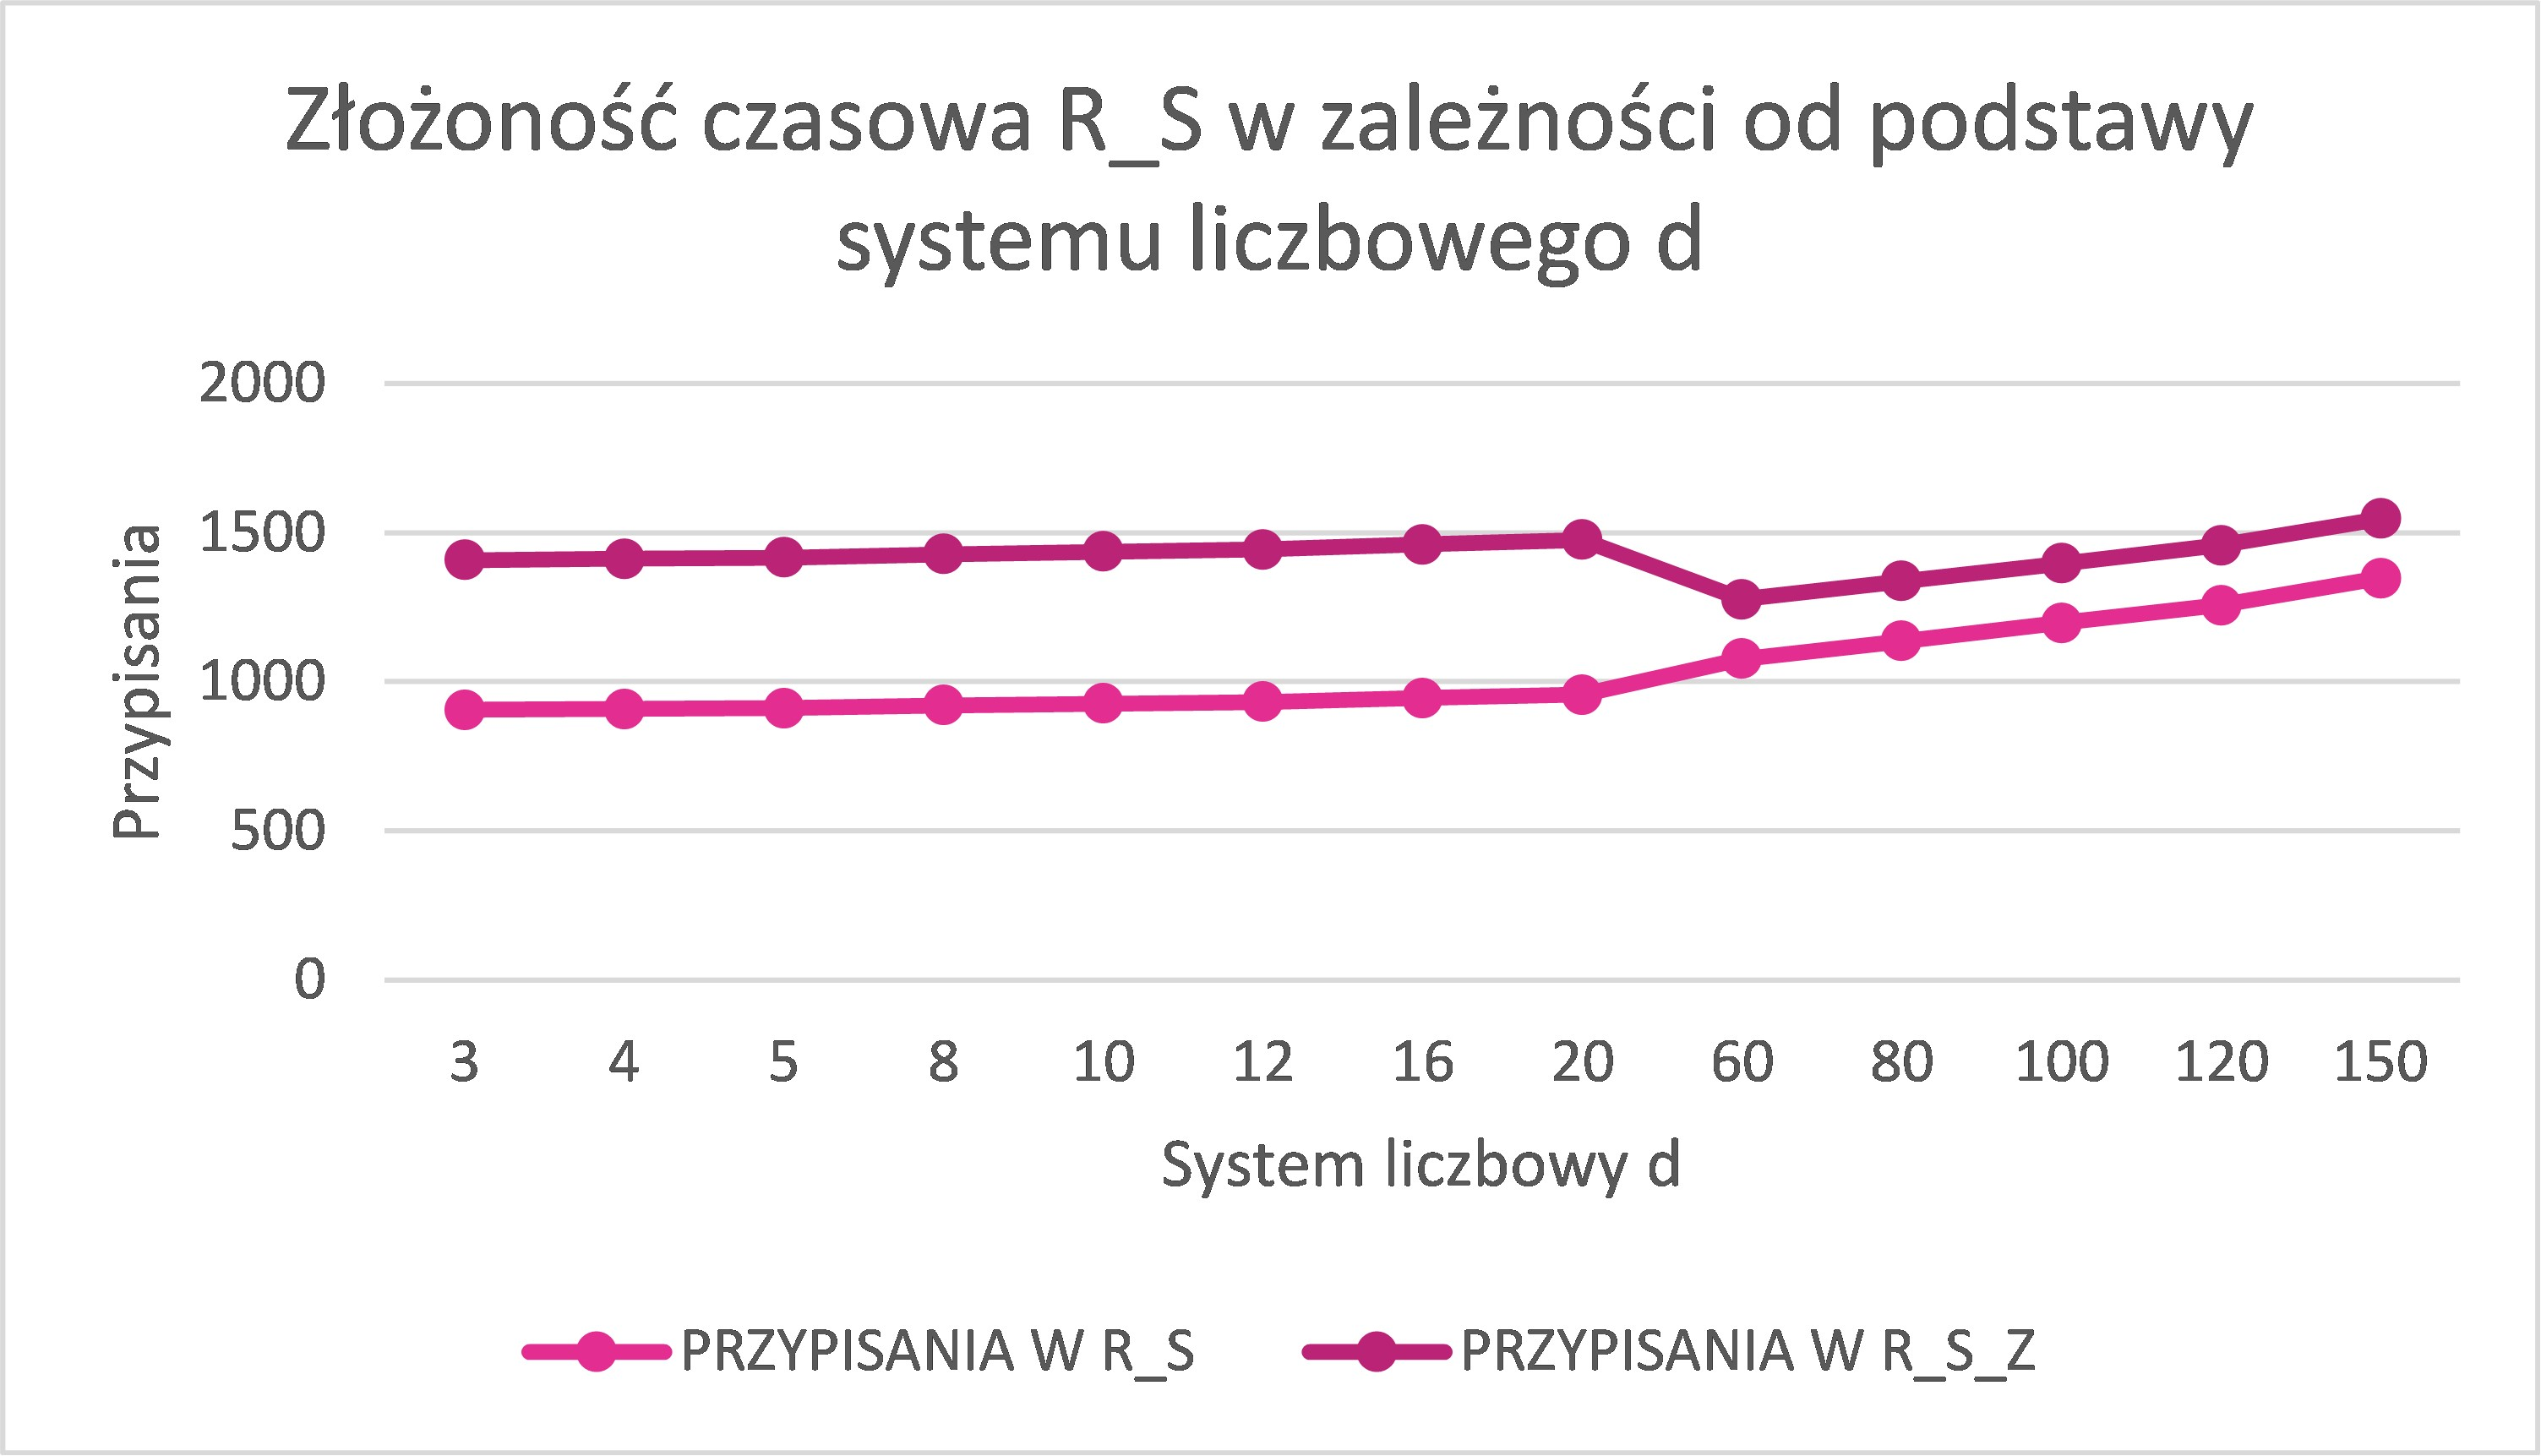
\includegraphics[width = \textwidth]{Obraz2.jpg}
	\end{center} 
	\section*{WNIOSKI}
	Jak widać na wykresie RADIXSORT działa dość stabilnie względem podstawy systemu liczbowego. Modyfikacja wykonuje się dłużej ze względu na występowanie w listach, na których była testowana, liczb ujemnych. Dodatkowe przypisania pozwalają dostosować dane do sortowania.
	\subsection*{PORÓWNANIE QS I BS W ZALEŻNOŚCI OD DŁUGOŚCI LISTY}
	\begin{center}
		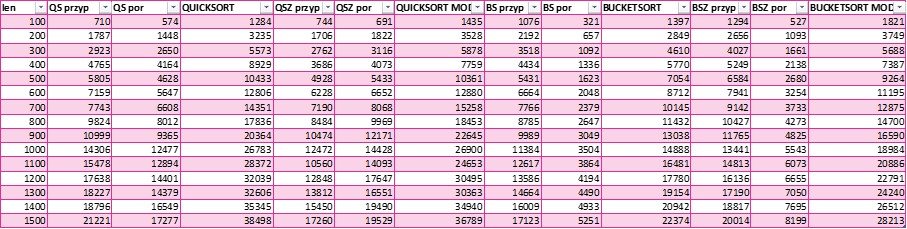
\includegraphics[width = \textwidth]{Obraz3.jpg}
	\end{center} 
	\begin{center}
		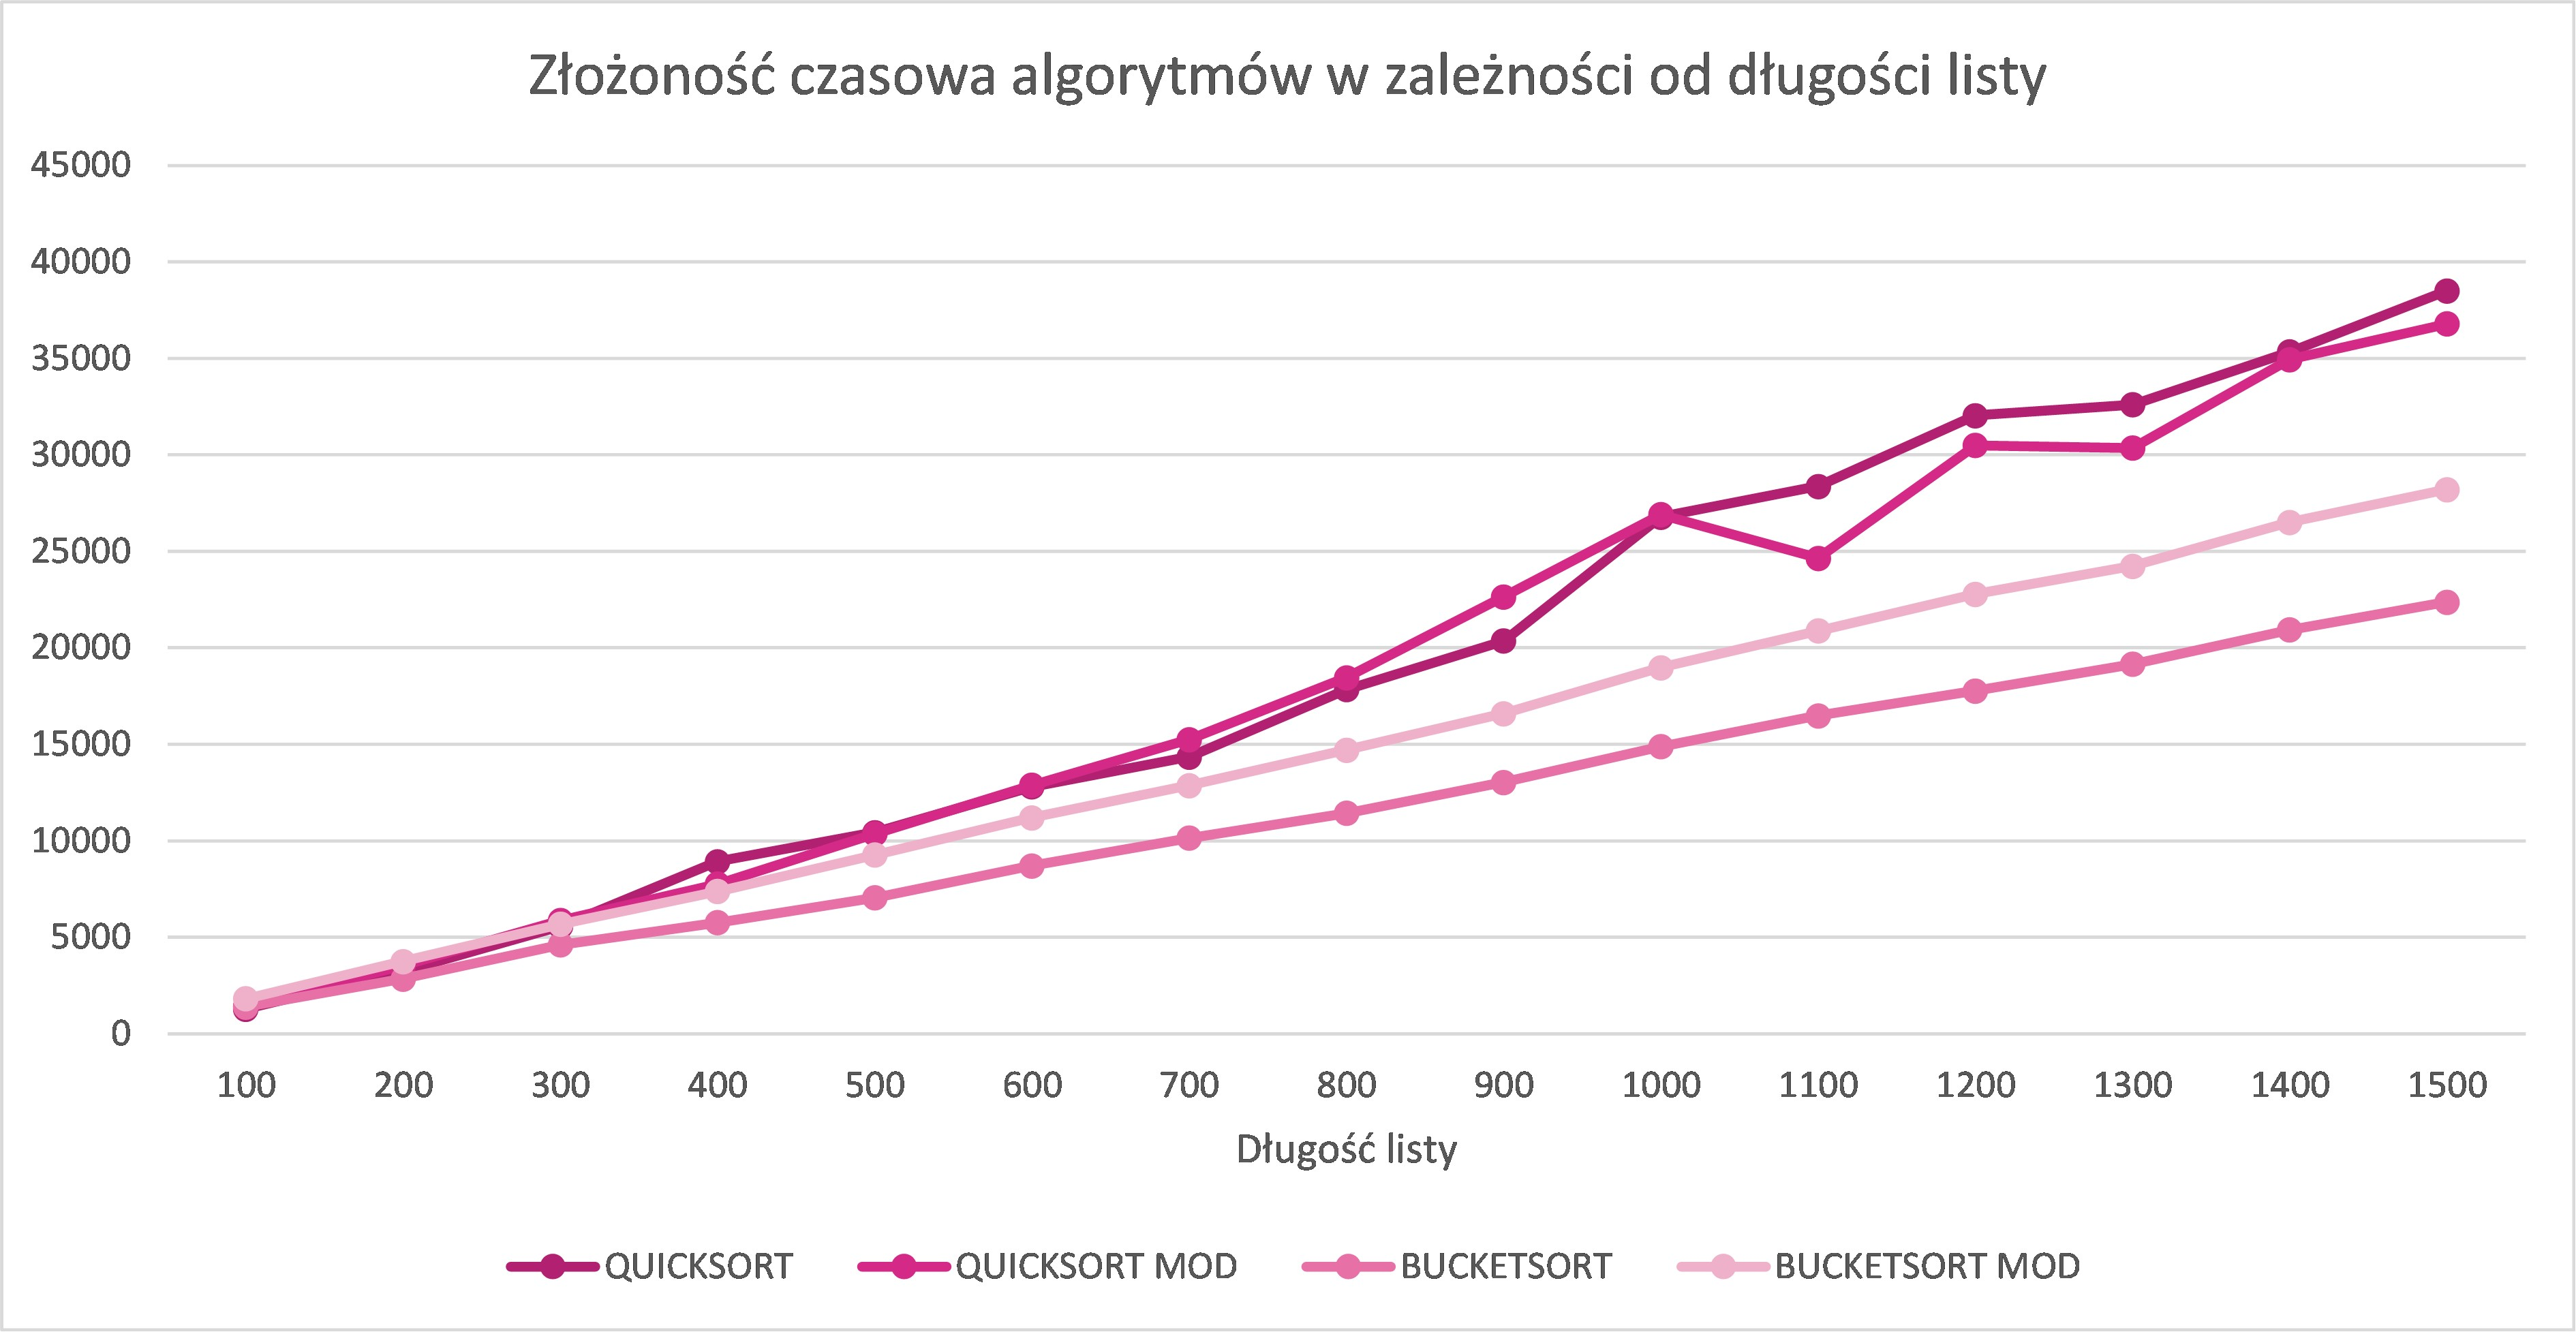
\includegraphics[width = \textwidth]{Obraz4.jpg}
	\end{center}
	\section*{WNIOSKI}
	Z wykresu wynika, że BUCKETSORT działa zarówno szybciej jak i stabilniej niż QUICKSORT. Modyfikacja QUICKSORT nieznacznie skraca czas działania algorytmu, zwłaszcza dla dłuższych list. Wykonuje ona mniej przypisań, ale kosztem ilości porównań. Modyfikacja BUCKETSORT nadal jest szybsza od QUICKSORT, a pozwala na sortowanie dowolnych wartości, w przeciwieństwie do pierwszej wersji, która sortuje wyłącznie wartści dodatnie.
\end{document}